\documentclass[11pt, a4paper, spanish, openright, twoside]{book}
\usepackage[spanish, activeacute]{babel}
\usepackage[utf8]{inputenc}
%\usepackage[top=2.5cm, bottom=2.5cm, outer=1.75cm, inner=1.75cm, heightrounded, marginparwidth=2.5cm, marginparsep=0.3cm]{geometry}	%márgenes empequeñecidos
\usepackage[top=2.95cm, bottom=2.25cm, outer=2.75cm, inner=2.75cm, heightrounded, marginparwidth=2.5cm, marginparsep=0.3cm]{geometry}	%márgenes originalmente
\usepackage{dpg}
\usepackage{fli}

\usepackage{pgf}
\usepackage{tikz}

\usepgflibrary{shapes.geometric} % LATEX and plain TEX and pure pgf
\usetikzlibrary{arrows,automata,positioning}
\tikzstyle{accepting by double}= [double distance=1.6pt,double,outer sep=.5\pgflinewidth+.8pt] % esto es algo estético.
\renewcommand\shorthandsspanish{}  % para compatibilizar spanish con tikz

%%%%%%		Figuras		%%%%%%%%%%%%%%%%%%%
\usepackage[vflt]{floatflt}		%Entorno float-figure

%%%%%%		Page style		%%%%%%%%%%%%%%%%%%%
\renewcommand{\thepage}{\arabic{page}}% Arabic page numbers\fancyhead{}
\pagestyle{fancy}
\fancyfoot{}
\fancyhead[LO,RE]{Práctica 7}	%encabezado de pares: nombre de la sección
\fancyhead[RO,LE]{Representación de conocimiento en \textbf{Prolog}}
\fancyfoot[LE,RO]{\thepage}	%abajo a izqda en pares, derecha en impares: numero de pagina
%\fancyhead[LE]{\nouppercase{\leftmark}} %cuadro izquierdo de pagina par: parte y contador
\fancyfoot[CE]{Inteligencia Artificial} 
\fancyfoot[CO]{Doble Grado Informática-Matemáticas - Universidad Complutense}
\renewcommand{\footrulewidth}{0.4pt}
\renewcommand{\headrulewidth}{0.4pt}		% linea por debajo del encabezado
\renewcommand{\sectionmark}[1]{\markright{\textbf{\thesection. #1}}}	%negrita
\renewcommand{\labelitemi}{$\circ$} %Primer itemize con circunferencia vacia
\renewcommand{\labelitemii}{$\cdot$} %Segundo itemize con punto pequeño \cdot
\renewcommand*{\thesection}{\arabic{section}}	% Hace que no apareca el indice de capitulos y que comience en section

%%%%%%		Others		%%%%%%%%%%%%%%%%%%%
\setlength{\leftmarginii}{0em} %Segundo itemize sin sangria
\setlength{\leftmarginiii}{1em} %Tercer itemize casi sin sangria
\renewcommand{\labelitemiii}{ }
\pagenumbering{roman}
\addto{\captionsspanish}{\renewcommand*{\contentsname}{Índice}} %Cambia "Indice general" por "Indice"



\begin{document} 
\title{\Huge{\textsc{Inteligencia Artificial}} \\
	\vspace{0.7cm}
	 \textsc{\Large{Práctica 7}} \\
	\vspace{1.5cm}
	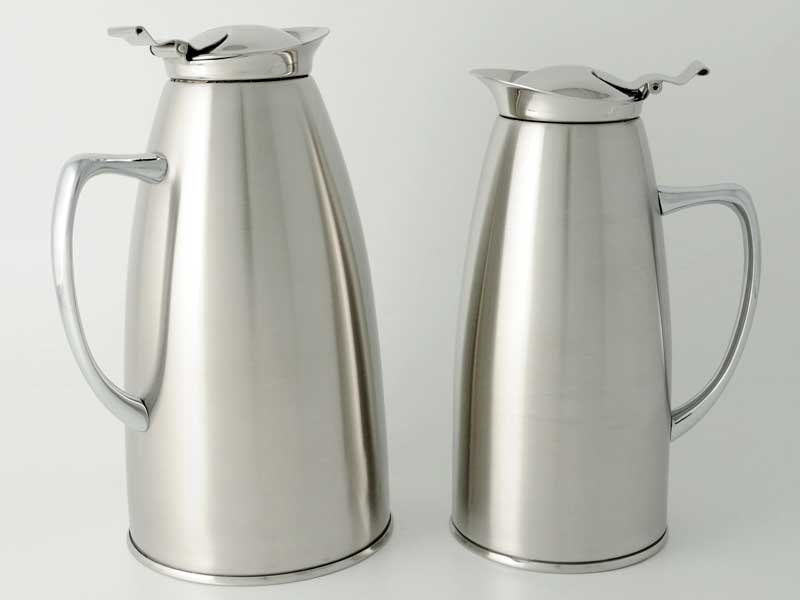
\includegraphics[scale=0.45]{jarras}}
\author{\textsc{Grupo 3:}\\
	Enrique Ballesteros Horcajo\\
	Ignacio Iker Prado Rujas}
\date{\Today}
\maketitle

\newpage
\mbox{}
\thispagestyle{empty}						% Hoja en blanco, sin numeros ni nada
\newpage


\tableofcontents 							%INDICE hipervinculado

\newpage
\mbox{}
\thispagestyle{empty}						% Hoja en blanco, sin numeros ni nada
\newpage

\pagenumbering{arabic}						% Pone el contador de paginas a 1 y ahora en numeros normales

\vspace{3cm}


\newpage



\begin{section}{Diferencias entre \textbf{Prolog} y \textbf{Jess}}
		En \textbf{Jess} se define un espacio concreto para los hechos iniciales (\texttt{deffacts ini}), mientras que en \textbf{Prolog} no es necesario debido a que es procedimental, lo cual nos permite que 
		al declarar los hechos iniciales al principio sean estos los que primero se añadan.
		Por tanto en \textbf{Jess} distinguimos explícitamente las reglas de los hechos, utilizando el \texttt{deffrule} y dándole un nombre concreto a la regla (que puede ser distinto del \texttt{assert} que se defina). En \textbf{Prolog} las reglas 
		y los hechos no se diferencian explícitamente. De hecho, al escribir  \texttt{dd(juan, maria, rosa, m).} estamos definiendo la regla \texttt{dd(juan, maria, rosa, m) :- true.}, que por supuesto se cumple siempre (no tiene premisas).
		
		La principal diferencia que hemos notado está en la recursión, ya  que en \textbf{Prolog} requiere colocar la llamada recursiva en la parte derecha de la sentencia (i.e., evitamos la recursión a al izquierda) porque resuelve la recursión en orden. En \textbf{Jess} no es estrictamente necesario hacer esto.
      
      Además, la sintaxis concreta es diferente: en \textbf{Prolog} se usa \texttt{X \textbackslash = Y} para el distinto y $\_$ para cualquiera. En cambio, en \textbf{Jess}, se utiliza \texttt{test (neq ?x ?y)} y \texttt{?} respectivamente, además de otras diferencias sintánticas más supérfluas. No es baladí mencionar que en \textbf{Jess} el consecuente se encuentra a continuación del antecedente, mientras que en \texttt{Prolog} la conclusión se encuentra antes que las premisas. Esto se debe a que primero permite encadenamiento progresivo y regresivo (aunque sea más sencillo usar el progresivo) y el segundo regresivo.

\begin{center}
	\includegraphics[scale=1.25]{prolog}
\end{center}
	
\end{section}
	\newpage
	\begin{section}{Algoritmo usado por Prolog}

		Sabemos que \textbf{Prolog} se ejecuta de manera procedimental, por lo que realiza las operaciones en el orden en que están escritas. Cambiando el orden de los operadores obtenemos primero diferentes soluciones, que estudiamos a continuación.

		\begin{subsection}{Ejecuciones con órdenes distintos en los operadores}
			Para el orden \texttt{llenar3, llenar4, verter3, verter4, vaciar3, vaciar4} las soluciones sucesivas van aumentando de longitud:

			\texttt{[llenar3,llenar4,vaciar3,verter4,vaciar3,verter4,llenar4,verter4] 8}
         
			\texttt{[llenar3,llenar4,vaciar3,verter4,vaciar3,verter4,llenar4,verter4,vaciar3] 9}
			
      \texttt{[llenar3,llenar4,vaciar3,verter4,vaciar3,verter4,verter3,verter4,llenar4,verter4] 10}
			
			Además, encuentra la solución óptima en el decimo séptimo intento.

			Para el orden \texttt{llenar3, verter3, vaciar4, llenar4, verter4 vaciar3} obtenemos la solución óptima en la quinta iteración: 
			
			\texttt{[llenar3,verter3,llenar3,verter3,vaciar4,verter3]  6}
         
			
		\end{subsection}

		Así, observamos que explora en profundidad con \textit{backtracking}, pues las soluciones que va encontrando de manera consecutiva tienen las primeras operaciones idénticas. Además, 
		sigue el orden de exploración en el que colocamos la deficición de las operaciones. Es un método no informado, pues no utilizamos ninguna heurística. 

La profundidad no está acotada 
		pues explora hasta haber visitado todos los estados posibles incluso a partir de soluciones encontradas. Lo único que controlamos es que no se repitan estados, pues en muchos casos podríamos tener una secuencia infinita (por ejemplo si las primeras dos operaciones fueses llenar3 y vaciar3, sin control de repeticiones se quedaría alternando entre ambas sin parar). Es decir, que sin este control sería una búsqueda 
		primero en profundidad, pues no encuentra la solución óptima y puede entrar en caminos infinitos. 

Concluímos pues que como controlamos las repeticiones es ``primero en profundidad $+$ control de repeticiones''.

	
	\end{section}

	
\begin{thebibliography}{9}

\bibitem{aima}
	Russell, S.; Norvig, P, \\
	\emph{Artificial Intelligence, a modern aproach}.\\
	New Jersey: Pearson, 2010.
	
\bibitem{clase}
	Apuntes y transparencias de Inteligencia Artificial, \\
	Doble Grado Matemáticas - Ing. Informática, U.C.M., 2014-2015.

\end{thebibliography}


\end{document}